\chapterimage{chapter_head_1.pdf}
\chapter{Conditionals}

\section{Modulus operator}

\index{modulus operator}
\index{operator!modulus}

The {\bf modulus operator} works on integers and yields the remainder
when the first operand is divided by the second.  In Python, the
modulus operator is a percent sign (\verb"%").  The syntax is the same
as for other operators:

\beforeverb
\begin{pyinterpreter}
>>> quotient = 7 // 3
>>> print(quotient)
2
>>> remainder = 7 % 3
>>> print(remainder)
1
\end{pyinterpreter}
\afterverb
%
So 7 divided by 3 is 2 with 1 left over.

The modulus operator turns out to be surprisingly useful.  For
example, you can check whether one number is divisible by another---if
{\tt x \% y} is zero, then {\tt x} is divisible by {\tt y}.
%
\index{divisibility}
%
Also, you can extract the right-most digit
or digits from a number.  For example, {\tt x \% 10} yields the
right-most digit of {\tt x} (in base 10).  Similarly {\tt x \% 100}
yields the last two digits.


\section{Boolean expressions}
\index{boolean expression}
\index{expression!boolean}
\index{logical operator}
\index{operator!logical}

A {\bf boolean expression} is an expression that is either true
or false.  The following examples use the 
operator {\tt ==}, which compares two operands and produces
{\tt True} if they are equal and {\tt False} otherwise:

\beforeverb
\begin{pyinterpreter}
>>> 5 == 5
True
>>> 5 == 6
False
\end{pyinterpreter}
\afterverb
%
{\tt True} and {\tt False} are special
values that belong to the type {\tt bool}; they are not strings:

\index{True special value}
\index{False special value}
\index{special value!True}
\index{special value!False}
\index{bool type}
\index{type!bool}

\beforeverb
\begin{pyinterpreter}
>>> type(True)
<type 'bool'>
>>> type(False)
<type 'bool'>
\end{pyinterpreter}
\afterverb
%
The {\tt ==} operator is one of the {\bf relational operators}; the
others are:

\beforeverb
\begin{pycode}
x != y               # x is not equal to y
x > y                # x is greater than y
x < y                # x is less than y
x >= y               # x is greater than or equal to y
x <= y               # x is less than or equal to y
\end{pycode}
\afterverb
%
Although these operations are probably familiar to you, the Python
symbols are different from the mathematical symbols.  A common error
is to use a single equal sign ({\tt =}) instead of a double equal sign
({\tt ==}).  Remember that {\tt =} is an assignment operator and
{\tt ==} is a relational operator.   There is no such thing as
{\tt =<} or {\tt =>}.

\index{relational operator}
\index{operator!relational}


\section {Logical operators}
\index{logical operator}
\index{operator!logical}

There are three {\bf logical operators}: {\tt and}, {\tt
or}, and {\tt not}.  The semantics (meaning) of these operators is
similar to their meaning in English. If you are not familiar with the logical operators, their {\bf truth table} are given in Table~\ref{tab:truth_table}. The tables read as follow, the operands value are given in the first row and first column. The operator is given in the first cell (top-left) of the table. Looking at the {\tt and} operator, the result of the expression {\tt True and True} is {\tt True}, whereas the result of the expression {\tt True and False} is {\tt False}.

\begin{table}[htb]
\begin{center}
\begin{minipage}[t]{.3\textwidth}
\begin{tabular}{|c|cc|}
\hline
and   & True  & False \\\hline
True  & True  & False \\
False & False & False \\\hline
\end{tabular}
\end{minipage}
%
\begin{minipage}[t]{.3\textwidth}
\begin{tabular}{|c|cc|}
\hline
or    & True  & False \\\hline
True  & True  & True  \\
False & True  & False \\\hline
\end{tabular}
\end{minipage}
%
\begin{minipage}[t]{.3\textwidth}
\begin{tabular}{|c|cc|}
\hline
not  & True  & False\\\hline
     & False & True \\\hline
\end{tabular}
\end{minipage}
%
\caption{Truth table for the three logical operators {\tt and}, {\tt or}, and {\tt not}.}
\label{tab:truth_table}
\end{center}
\end{table}

%
\index{and operator}
\index{or operator}
\index{not operator}
\index{operator!and}
\index{operator!or}
\index{operator!not}
\index{operator!truth table}

%
 For example, {\tt x > 0 and x < 10} is true only if {\tt x} is greater than 0
{\em and} less than 10. Another example, {\tt n\%2 == 0 or n\%3 == 0} is true if {\em either} of the conditions
is true, that is, if the number is divisible by 2 {\em or} 3.
%
Finally, the {\tt not} operator negates a Boolean
expression, so {\tt not (x > y)} is true if {\tt x > y} is false,
that is, if {\tt x} is less than or equal to {\tt y}.

\begin{remark}
Strictly speaking, the operands of the logical operators should be
Boolean expressions, but Python is not very strict.
Any nonzero number is interpreted as ``true'', wheres as 0 is interpreted as ``false''.

\beforeverb
\begin{pyinterpreter}
>>> 17 and True
True
\end{pyinterpreter}
\afterverb
%
This flexibility can be useful, but there are some subtleties to
it that might be confusing.  You might want to (shall I say MUST) avoid it, even if
you know what you are doing. Another developer maintaining your code may not be familiar with the subtleties.

\end{remark}


\section{Conditional execution}
\label{conditional execution}

\index{conditional statement}
\index{statement!conditional}
\index{if statement}
\index{statement!if}
\index{conditional execution}

In order to write useful programs, we almost always need the ability
to check conditions and change the behavior of the program
accordingly.  {\bf Conditional statements} give us this ability.  The
simplest form is the {\tt if} statement:

\beforeverb
\begin{pycode}
if x > 0:
    print('x is positive')
\end{pycode}
\afterverb
%
The Boolean expression after the {\tt if} statement is
called the {\bf condition}.  If it is true, then the indented
statement gets executed.  If not, nothing happens. This is illustrated in the flow diagram shown in Figure~\ref{fig:if-statement}.

\begin{figure}[htb]%
\begin{center}
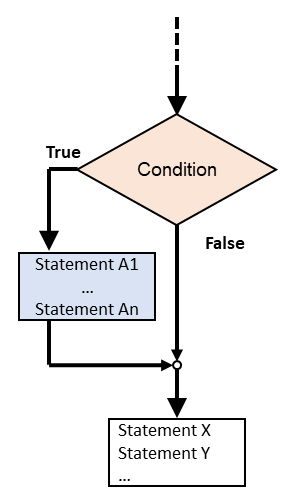
\includegraphics[height=7cm]{figs/ifstatementdiagram.png}%
\caption{Conditional {\tt if} statement control flow diagram.}%
\label{fig:if-statement}%
\end{center}
\end{figure}

\index{flow diagram!if statement}
\index{condition}
\index{compound statement}
\index{statement!compound}

{\tt if} statements have the same structure as function definitions:
a header followed by an indented body.  Statements like this are
called {\bf compound statements}.
%
There is no limit on the number of statements that can appear in
the body, but there has to be at least one.
Occasionally, it is useful to have a body with no statements (usually
as a place keeper for code you haven't written yet).  In that
case, you can use the {\tt pass} statement, which does nothing.

\index{pass statement}
\index{statement!pass}

\beforeverb
\begin{pycode}
if x < 0:
    pass          # need to handle negative values!
\end{pycode}
\afterverb
%

\section{Alternative execution}
\label{alternative execution}

\index{alternative execution}
\index{else keyword}
\index{keyword!else}

A second form of the {\tt if} statement is {\bf alternative execution} (aka {\tt if-else} statement),
in which there are two possibilities and the condition determines
which one gets executed.  The syntax looks like this:

\beforeverb
\begin{pycode}
if x%2 == 0:
    print('x is even')
else:
    print('x is odd')
\end{pycode}
\afterverb
%
If the remainder when {\tt x} is divided by 2 is 0, then we
know that {\tt x} is even, and the program displays a message to that
effect.  If the condition is false, the second set of statements is
executed.  Since the condition must be true or false, exactly one of
the alternatives will be executed.  The alternatives are called
{\bf branches}, because they are branches in the flow of execution.
This is clearly illustrated in the flow diagram shown in Figure~\ref{fig:if-else-statement}.

\index{branch}
\index{flow diagram!if-else statement}

\begin{figure}[htb]%
\begin{center}
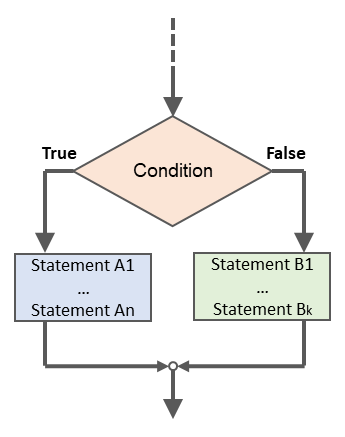
\includegraphics[height=7cm]{figs/ifelsestatementdiagram.png}%
\caption{Conditional {\tt if-else} statement control flow diagram.}%
\label{fig:if-else-statement}%
\end{center}
\end{figure}



\section{Chained conditionals}
\index{chained conditional}
\index{conditional!chained}

Sometimes there are more than two possibilities and we need more than
two branches.  One way to express a computation like that is a {\bf
chained conditional} (aka {\tt if-elif-else} statement):

\beforeverb
\begin{pycode}
if x < y:
    print('x is less than y')
elif x > y:
    print('x is greater than y')
else:
    print('x and y are equal')
\end{pycode}
\afterverb
%
{\tt elif} is an abbreviation of ``else if.''  Again, exactly one
branch will be executed.  There is no limit on the number of {\tt
elif} statements.  If there is an {\tt else} clause, it has to be
at the end, but there doesn't have to be one.

\index{elif keyword}
\index{keyword!elif}


\beforeverb
\begin{pycode}
if choice == 'a':
    draw_a()
elif choice == 'b':
    draw_b()
elif choice == 'c':
    draw_c()
\end{pycode}
\afterverb
%
Each condition is checked in order.  If the first is false,
the next is checked, and so on.  If one of them is
true, the corresponding branch executes, and the statement
ends.  Even if more than one condition is true, only the
first true branch executes.  The flow diagram of a chained 
conditional is shown in Figure~\ref{fig:if-elif-statement}.

\index{branch}
\index{flow diagram!if-elif-else statement}

\begin{figure}[htb]%
\begin{center}
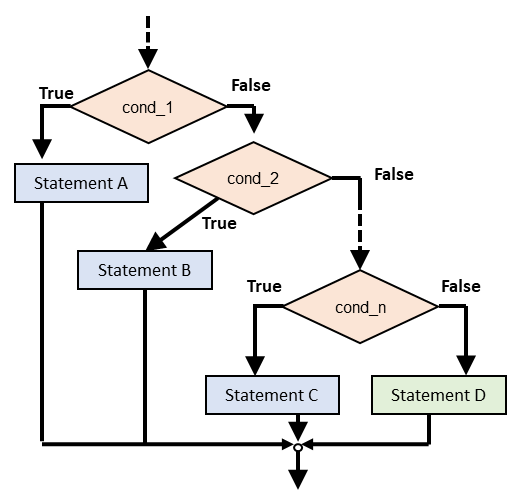
\includegraphics[height=8cm]{figs/ifelifstatementdiagram.png}%
\caption{Conditional {\tt if-elif-else} statement control flow diagram.}%
\label{fig:if-elif-statement}%
\end{center}
\end{figure}


\section{Nested conditionals}
\index{nested conditional}
\index{conditional!nested}

One conditional can also be nested within another.  We could have
written the trichotomy example like this:

\beforeverb
\begin{pycode}
if x == y:
    print('x and y are equal')
else:
    if x < y:
        print('x is less than y')
    else:
        print('x is greater than y')
\end{pycode}
\afterverb
%
The outer conditional contains two branches.  The
first branch contains a simple statement.  The second branch
contains another {\tt if} statement, which has two branches of its
own.  Those two branches are both simple statements,
although they could have been conditional statements as well.
%
Although the indentation of the statements makes the structure
apparent, {\bf nested conditionals} become difficult to read very
quickly. In general, it is a good idea to avoid them when you can.

Nested conditionals structures should be used when several statements are
common to more than one sub-branch as illustrated in Figure~\ref{fig:nested-if-statements}. 
Here, statements {\tt B1} and {\tt B2} have been moved out of the nested {\tt if} statement as if is common to branches {\tt C} and {\tt D}. The same flow of execution could have been done using chained conditionals, however statements {\tt B1} and {\tt B2} would have to be duplicate in each sub-branch.

\index{flow diagram!nested if statements}

\begin{figure}[htb]%
\begin{center}
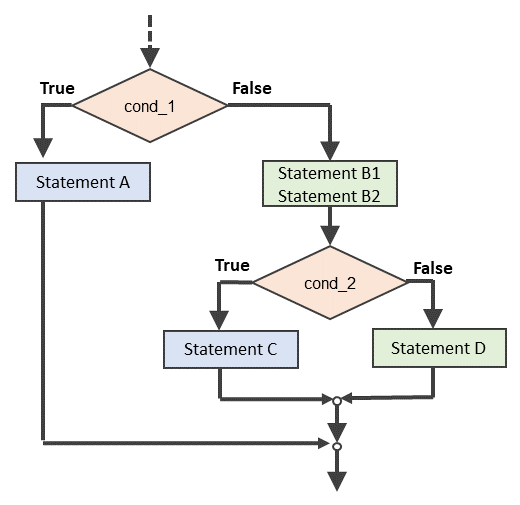
\includegraphics[height=8cm]{figs/ifnestedstatementsdiagram.png}%
\caption{Nested conditionals {\tt if} statements control flow diagram.}%
\label{fig:nested-if-statements}%
\end{center}
\end{figure}



Logical operators often provide a way to simplify nested conditional
statements.  For example, we can rewrite the following code using a
single conditional:

\beforeverb
\begin{pycode}
if 0 < x:
    if x < 10:
        print('x is a positive single-digit number.')
\end{pycode}
\afterverb
%
The {\tt print} statement is executed only if we make it past both
conditionals, so we can get the same effect with the {\tt and} operator:

\beforeverb
\begin{pycode}
if 0 < x and x < 10:
    print('x is a positive single-digit number.')
\end{pycode}
\afterverb		


